\documentclass[handout]{beamer}
%\documentclass{beamer}
\usepackage{tikz}
\def\checkmark{\tikz\fill[scale=0.4](0,.35) -- (.25,0) -- (1,.7) -- (.25,.15) -- cycle;} 
\usepackage{pifont}
\newcommand{\xmark}{\ding{55}}
\usepackage{tikz}
\usepackage{biblatex}
\usetheme{PaloAlto}
\title{Hamiltonian Monte Carlo and how to speak Stan}
\author[Ben Lambert]{Ben Lambert\inst{1}\\ \texttt{ben.lambert@stats.ox.ac.uk}}
\beamertemplatenavigationsymbolsempty
\setbeamertemplate{sidebar left}{}
\usepackage{caption}
\captionsetup{font=footnotesize}
\usepackage[utf8]{inputenc}
\usepackage{amsmath}
\usepackage{multimedia}
\usepackage{animate}
\usepackage{graphics}
\usepackage{graphicx}
\usepackage[makeroom]{cancel}
\usepackage{relsize}
\usepackage{listings}
\usepackage[]{graphicx}\usepackage[]{color}
\usepackage{minted}
%% maxwidth is the original width if it is less than linewidth
%% otherwise use linewidth (to make sure the graphics do not exceed the margin)
\makeatletter
\def\maxwidth{ %
	\ifdim\Gin@nat@width>\linewidth
	\linewidth
	\else
	\Gin@nat@width
	\fi
}
\makeatother

\definecolor{fgcolor}{rgb}{0.345, 0.345, 0.345}
\newcommand{\hlnum}[1]{\textcolor[rgb]{0.686,0.059,0.569}{#1}}%
\newcommand{\hlstr}[1]{\textcolor[rgb]{0.192,0.494,0.8}{#1}}%
\newcommand{\hlcom}[1]{\textcolor[rgb]{0.678,0.584,0.686}{\textit{#1}}}%
\newcommand{\hlopt}[1]{\textcolor[rgb]{0,0,0}{#1}}%
\newcommand{\hlstd}[1]{\textcolor[rgb]{0.345,0.345,0.345}{#1}}%
\newcommand{\hlkwa}[1]{\textcolor[rgb]{0.161,0.373,0.58}{\textbf{#1}}}%
\newcommand{\hlkwb}[1]{\textcolor[rgb]{0.69,0.353,0.396}{#1}}%
\newcommand{\hlkwc}[1]{\textcolor[rgb]{0.333,0.667,0.333}{#1}}%
\newcommand{\hlkwd}[1]{\textcolor[rgb]{0.737,0.353,0.396}{\textbf{#1}}}%

\usepackage{framed}
\makeatletter
\newenvironment{kframe}{%
	\def\at@end@of@kframe{}%
	\ifinner\ifhmode%
	\def\at@end@of@kframe{\end{minipage}}%
\begin{minipage}{\columnwidth}%
	\fi\fi%
	\def\FrameCommand##1{\hskip\@totalleftmargin \hskip-\fboxsep
		\colorbox{shadecolor}{##1}\hskip-\fboxsep
		% There is no \\@totalrightmargin, so:
		\hskip-\linewidth \hskip-\@totalleftmargin \hskip\columnwidth}%
	\MakeFramed {\advance\hsize-\width
		\@totalleftmargin\z@ \linewidth\hsize
		\@setminipage}}%
{\par\unskip\endMakeFramed%
	\at@end@of@kframe}
\makeatother

\usepackage{xcolor}
\definecolor{orangeBright}{RGB}{243,146,0}
\definecolor{blueBright}{RGB}{54,169,225}
\definecolor{pinkBright}{RGB}{214,11,82}
\definecolor{shadecolor}{rgb}{.97, .97, .97}
\definecolor{messagecolor}{rgb}{0, 0, 0}
\definecolor{warningcolor}{rgb}{1, 0, 1}
\definecolor{errorcolor}{rgb}{1, 0, 0}
\newenvironment{knitrout}{}{} % an empty environment to be redefined in TeX

\usepackage{alltt}
\IfFileExists{upquote.sty}{\usepackage{upquote}}{}

\lstset{
    literate={~} {$\sim$}{1}
}

\makeatletter
\newcommand\mathcircled[1]{%
  \mathpalette\@mathcircled{#1}%
}
\newcommand\@mathcircled[2]{%
  \tikz[baseline=(math.base)] \node[draw,circle,inner sep=1pt] (math) {$\m@th#1#2$};%
}
\makeatother

\bibliography{Bayes}

\begin{document}

\begin{frame}
\titlepage
\end{frame}

\begin{frame}
\frametitle{Lecture outcomes}

By the end of this lecture you should:
\begin{enumerate}
	\item<3-> Grasp the intuition behind Hamiltonian Monte Carlo, and the benefits of this algorithm.
	\item<4-> Know how to start coding up a model in Stan.
	\item<5-> Appreciate how easy Stan makes things for us compared to coding up the algorithm ourselves.
	\item<6-> Know what to do when coding goes wrong.
	\item<7-> Know what to do when sampling goes wrong.
\end{enumerate}

\end{frame}


\begin{frame}
	\frametitle{Effective sample size}
	\onslide<2->
	\textbf{Question:} How do we compare the performance of two sampling algorithms?
	
	\vspace{0.2cm}
	
	\onslide<3-> \textbf{Answer:} Estimate the number of effective samples per $X$ iterations,
	
	\onslide<4-> ``The \textbf{effective sample size} for $X$ iterations is the equivalent number of samples from an independent sampler.''  
	
\end{frame}

\begin{frame}
	\frametitle{Effective sample size}
	\onslide<2->
	\textbf{Question:} But how do we estimate the effective sample size?
	
	\vspace{0.2cm}
	
	\onslide<3->
	\textbf{Answer:} Design a metric so that as dependence $\rightarrow$ 0 $\implies$ effective sample size $\rightarrow$ actual sample size. \onslide<4-> But why does dependence matter?
\end{frame}

\begin{frame}
	\frametitle{Introducing a Markovian die}
	\onslide<2-> A standard die has six faces, all of which are equally likely to be obtained on a given throw.
	
	\onslide<1->
	\begin{figure}[ht]
		\centerline{\includegraphics[width=0.8\textwidth]{./Figures/dice1.pdf}}
	\end{figure}
	
\end{frame}

\begin{frame}
	\frametitle{Introducing a Markovian die}
	\onslide<2-> This can be represented in graphical form,
	
	\onslide<3->
	\begin{figure}[ht]
		\centerline{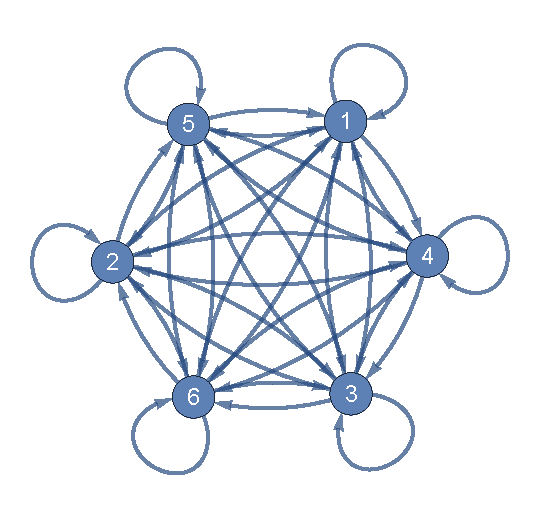
\includegraphics[width=0.75\textwidth]{./Figures/lec6_independentDie.pdf}}
	\end{figure}
	
\end{frame}

\begin{frame}
	\frametitle{Introducing a Markovian die}
	\onslide<2-> Now suppose we have a die where from each number only consecutive numbers can be obtained,
	
	\begin{itemize}
		\item<3-> $1\rightarrow 2$ or $1\rightarrow 6$; each with probability 1/2.
		\item<4-> $2\rightarrow 3$ or $2\rightarrow 1$; each with probability 1/2.
		\item<5-> ...
		\item<6-> $6\rightarrow 1$ or $6\rightarrow 5$; each with probability 1/2.
	\end{itemize}
	
	\onslide<7-> This die has \textbf{dependence} -- the next value we obtain depends on the current value!
	\onslide<8-> \textbf{However} has same unconditional distribution (i.e. across all throws) as independent die \onslide<9-> $\rightarrow$ same mean.
	
\end{frame}

\begin{frame}
	\frametitle{Introducing a Markovian die}
	\onslide<2-> This \textbf{Markovian} die can be represented in graphical form,
	
	\onslide<3->
	\begin{figure}[ht]
		\centerline{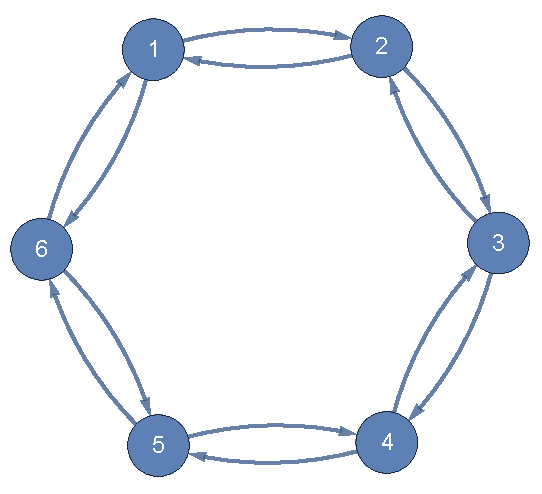
\includegraphics[width=0.75\textwidth]{./Figures/lec6_dependentDie.pdf}}
	\end{figure}
	
\end{frame}

\begin{frame}
	\frametitle{Introducing a Markovian die}
	\onslide<2-> \textbf{Question:} Which of these two dies -- the independent and Markovian one -- is better able to estimate the mean of the die?
	
	\onslide<3-> \textbf{Answer:} shake it off (again)!
	
	\onslide<1->
	\begin{figure}[ht]
		\centerline{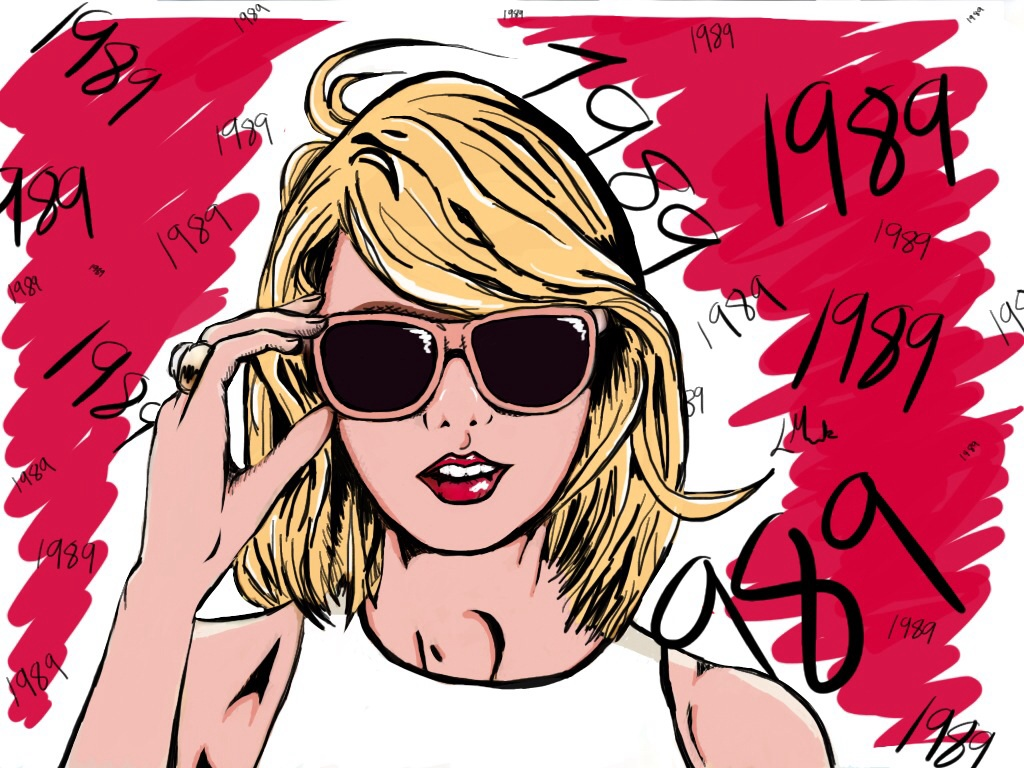
\includegraphics[width=1.0\textwidth]{./Figures/taylorSwift.jpg}}
	\end{figure}
	
\end{frame}


\begin{frame}
	\frametitle{Effective sample size: Markovian die}
	
\begin{figure}[t]
	\centerline{\animategraphics[width=0.9\textwidth,controls,buttonsize=1em,buttonfg=0.5]{2}{./Animations/lec6_markovDie_dependent}{1}{50}}
\end{figure}
	
\end{frame}

\begin{frame}
	\frametitle{Effective sample size: independent die}
	
	\begin{figure}[t]
		\centerline{\animategraphics[width=0.9\textwidth,controls,buttonsize=1em,buttonfg=0.5]{2}{./Animations/lec6_markovDie_independent}{1}{50}}
	\end{figure}
	
\end{frame}

\begin{frame}
	\frametitle{Effective sample size}
	\onslide<2-> \textbf{Conclude:} independent die converges more rapidly to true mean!
	
	
	\onslide<3-> 
	\textbf{Question:} How does each die fare in estimating any other quantity?
	
	\onslide<4->
	\vspace{0.2cm}
	\textbf{Answer:} Depends on how well each method approximates the probability distribution!
	
	
\end{frame}

\begin{frame}
	\frametitle{Effective sample size: Markovian die}
	
	\begin{figure}[t]
		\centerline{\animategraphics[width=0.9\textwidth,controls,buttonsize=1em,buttonfg=0.5]{2}{./Animations/lec6_markovDie_dependentHist}{1}{50}}
	\end{figure}
	
\end{frame}

\begin{frame}
	\frametitle{Effective sample size: independent die}
	
	\begin{figure}[t]
		\centerline{\animategraphics[width=0.9\textwidth,controls,buttonsize=1em,buttonfg=0.5]{2}{./Animations/lec6_markovDie_independentHist}{1}{50}}
	\end{figure}
	
\end{frame}

\begin{frame}
	\frametitle{Effective sample size: depends on dependence}
	\begin{itemize}
		\item<2-> The Markovian die performs worse than the independent sampler.
		\item<3-> This is due to the \textbf{dependence} of throwing the Markovian die \onslide<4-> $\implies$ takes longer for sampler to explore parameter space!
		\item<5-> As dependence$\uparrow$ the gap between the independent sampler and the Markovian one increases.
		\item<6-> Therefore conclude that as dependence$\uparrow$ the effective sample size $\downarrow$.
	\end{itemize}
	
	
\end{frame}


\begin{frame}
	\frametitle{Effective sample size: estimating for the Markovian die}
	\onslide<2-> \textbf{Question:} But how do we estimate effective sample size for a sample size of 50 from the Markovian die?
	
	\vspace{0.2cm}
	
	\onslide<3-> \textbf{Answer:} Estimate the error in estimating the mean (or another quantity if appropriate) for such a sample size, then find a sample size for the independent sampler that equilibrates the error.
	
\end{frame}

\begin{frame}
	\frametitle{Effective sample size:  estimating for the Markovian die}
	\onslide<2-> Across 10,000 samples, each of size 50, determine the error in estimating the mean,
	\onslide<4-> Root mean squared error ("average error") is $\approx 0.34$.   
	
	\onslide<3->
	\begin{figure}[ht]
		\centerline{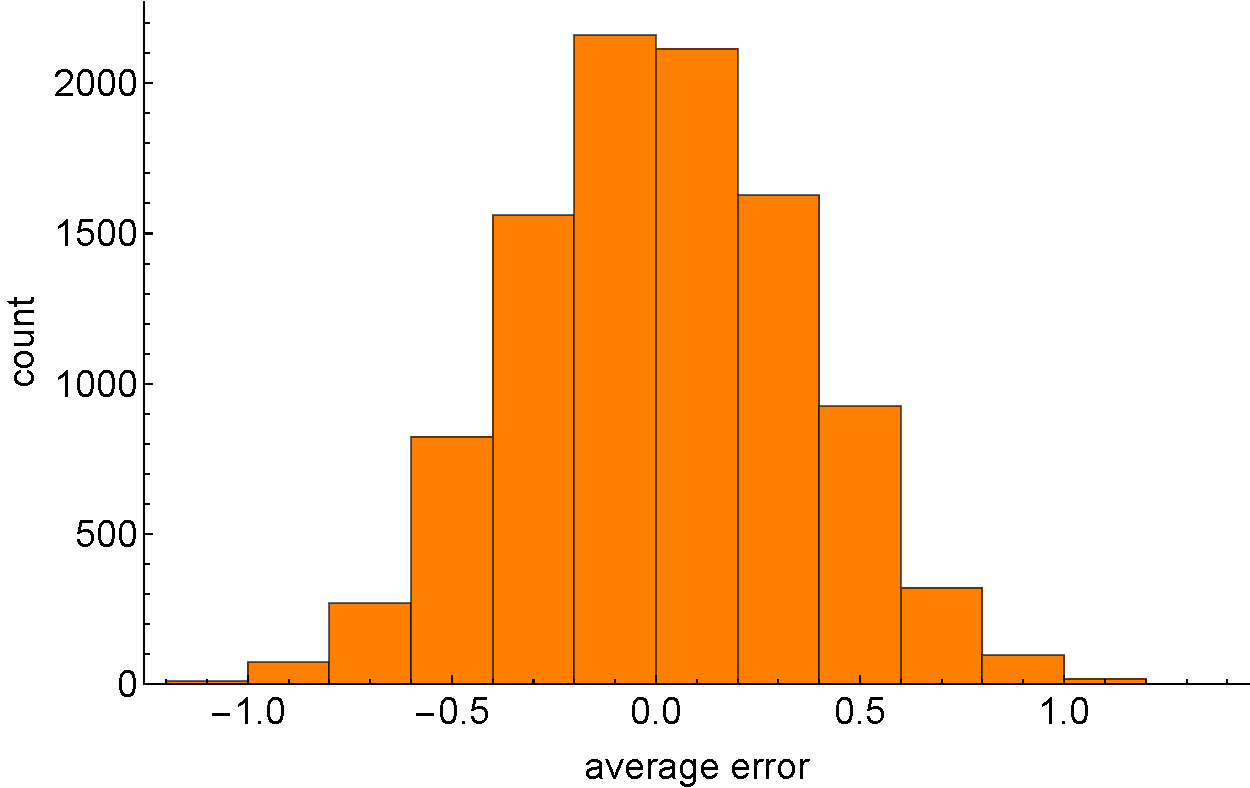
\includegraphics[width=0.85\textwidth]{./Figures/lec6_MarkovianDie_averageError.pdf}}
	\end{figure}
	
	
	
\end{frame}

\begin{frame}
	\frametitle{Effective sample size:  estimating for the Markovian die}
	\onslide<2-> Plot error of independent die as a function of sample size (again using 10,000 replicates of each sample size),
	\onslide<3->
	\begin{figure}[ht]
		\centerline{\includegraphics[width=0.8\textwidth]{./Figures/lec6_MarkovianDie_independentSampleSize1.pdf}}
	\end{figure}
	
\end{frame}

\begin{frame}
	\frametitle{Effective sample size:  estimating for the Markovian die}
	\onslide<1-> Find sample size that produces equivalent error for independent sampler \onslide<2-> $\rightarrow$ roughly 24, so independent sampler is about twice as efficient as Markovian die!
	\onslide<1->
	\begin{figure}[ht]
		\centerline{\includegraphics[width=0.8\textwidth]{./Figures/lec6_MarkovianDie_independentSampleSize2.pdf}}
	\end{figure}
	
\end{frame}

\begin{frame}
	\frametitle{Effective sample size: summary}
	\begin{itemize}
		\item<2-> The worth of a sample is \textbf{not} dictated by its number of samples per second.
		\item<3-> More important is the net information gained per second.
		\item<4-> As dependence of sampler increases there is less incremental information gained per sample.
		\item<5-> Quantify this using concept of effective sample size -- the equivalent number of samples from an independent sampler.
		\item<6-> Stan calculates this \textbf{automatically} for all parameters! No need to know formula.
	\end{itemize}
\end{frame}

\begin{frame}
	\frametitle{Defining the Gibbs sampler}
	
	\onslide<2-> For a parameter vector: $\boldsymbol{\theta} = (\theta_1,\theta_2,\theta_3)$:
	\begin{itemize}
		\item<3-> Select a random starting location: $(\textcolor{blue}{\theta^0_1},\textcolor{blue}{\theta^0_2},\textcolor{blue}{\theta^0_3})$, along the same lines as for Random Walk Metropolis.
		\item<4-> For each iteration $t = 1,...,T$ do:
		\begin{enumerate}
			\item<5-> Select a random parameter update ordering, for example $(\theta_3,\theta_2,\theta_1)$.
			\item<6-> \textbf{Independently} sample from the conditional posterior for each parameter in order using the most up-to-date parameters.
		\end{enumerate}
	\end{itemize}

\end{frame}

\begin{frame}
	\frametitle{Defining the Gibbs sampler}
	
	Start with $(\textcolor{blue}{\theta^0_1},\textcolor{blue}{\theta^0_2},\textcolor{blue}{\theta^0_3})$, then we sample:
	
	\onslide<2->
	\begin{equation}
	\textcolor{orange}{\theta^1_3}\sim p(\theta_3|\textcolor{blue}{\theta^0_2},\textcolor{blue}{\theta^0_1})
	\end{equation}
	
	\onslide<3-> Then conditional on freshly-sampled $\textcolor{orange}{\theta^1_3}$:
	\onslide<4->
	\begin{equation}
	\textcolor{orange}{\theta^1_2}\sim p(\theta_2|\textcolor{blue}{\theta^0_1},\textcolor{orange}{\theta^1_3})
	\end{equation}
	
	\onslide<5-> Then conditional on freshly-sampled $\textcolor{orange}{\theta^1_3}$ and $\textcolor{orange}{\theta^1_2}$:
	\onslide<6->
	
	\begin{equation}
	\textcolor{orange}{\theta^1_1}\sim p(\theta_1|\textcolor{orange}{\theta^1_2},\textcolor{orange}{\theta^1_3})
	\end{equation}
	
\end{frame}

\begin{frame}
	\frametitle{How to make a Gibbs sampler?}
	
	\begin{itemize}
		\item<2-> Typically better efficiency (i.e. higher effective sample size per iteration) than Random Walk Metropolis.
		\item<3-> Gibbs sampling requires that we derive \textbf{conditional} densities, for example $p(\theta_1|\theta_2,\theta_3)$.
		\item<4-> But how can we do find these densities in practice? (See problem set!)
		\item<5-> $\implies$ write down full posterior distribution, and take only those parts which involve the variable(s) that is being sampled.
		\item<6-> Then use knowledge of distributions to determine densities.
		\item<7-> Would prefer a method that didn't require us to do any maths!
	\end{itemize}
	
\end{frame}

\section{Introduction to Hamiltonian Monte Carlo}
\frame{\tableofcontents[currentsection]}

\begin{frame}
	\frametitle{Introduction to Hamiltonian Monte Carlo}
	\begin{itemize}
		\item<2-> Assume a space related to posterior space can be thought of as a landscape.
		\item<3-> Imagine an ice puck moving over the frictionless surface of this terrain.
		\item<4-> At defined time points we measure the location of the puck, and instantaneously give the puck a shove in a random direction.
		\item<5-> The locations traced out by the puck represent proposed steps from our sampler.
		\item<6-> Based on the height of the posterior and momentum of the puck we accept/reject steps.
	\end{itemize}
	
\end{frame}

\begin{frame}
	\frametitle{Why does this physical analogy help us?}
	
	\begin{figure}[ht]
		\centerline{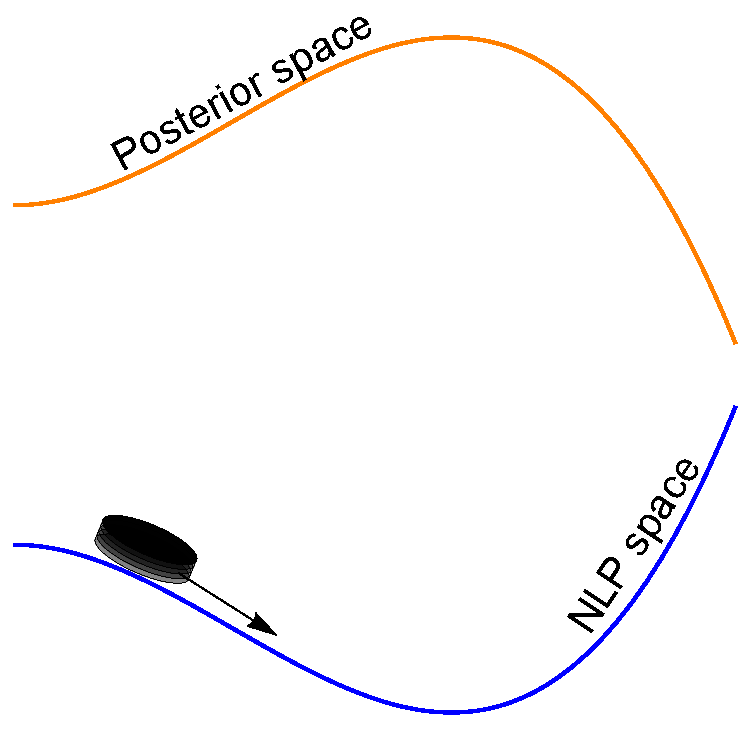
\includegraphics[width=0.7\textwidth]{./Figures/lec5_icePuck.pdf}}
	\end{figure}
	
\end{frame}

\begin{frame}
	\frametitle{Why does this physical analogy help us?}
	
	\begin{itemize}
		\item<2-> Allow the potential energy of the puck to be determined partly by the posterior density.
		\item<3-> $\implies$ puck will move in the ``natural'' directions dictated by the posterior geometry.
		\item<4-> And will visit areas of low NLP $\implies$ high posterior density.
		\item<5-> \textbf{NLP} stands for the \textbf{negative log (un-normalised) posterior},
		
		\begin{equation}
			NLP = - \text{log}\; \left[p(X|\theta) \times p(\theta) \right]
		\end{equation}
		
	\end{itemize}
	
	\onslide<6-> Important to remember that HMC uses the \textbf{log} of the posterior.
	
	\onslide<7-> (When coding up model in Stan ``sampling'' statements amount to incrementing the log probability.)
	
\end{frame}

\begin{frame}
	\frametitle{Simulating the puck's motion in NLP space: start with a posterior}
	
	\begin{figure}[ht]
		\centerline{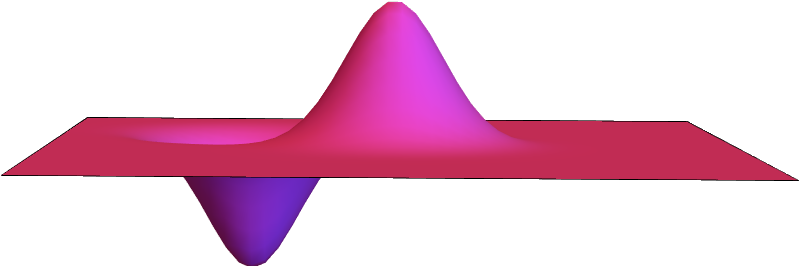
\includegraphics[width=1\textwidth]{./Figures/lec5_nlpPosteriorOnly.png}}
	\end{figure}
	
\end{frame}

\begin{frame}
	\frametitle{Simulating the puck's motion in NLP space: find NLP space}
	
	\begin{figure}[ht]
		\centerline{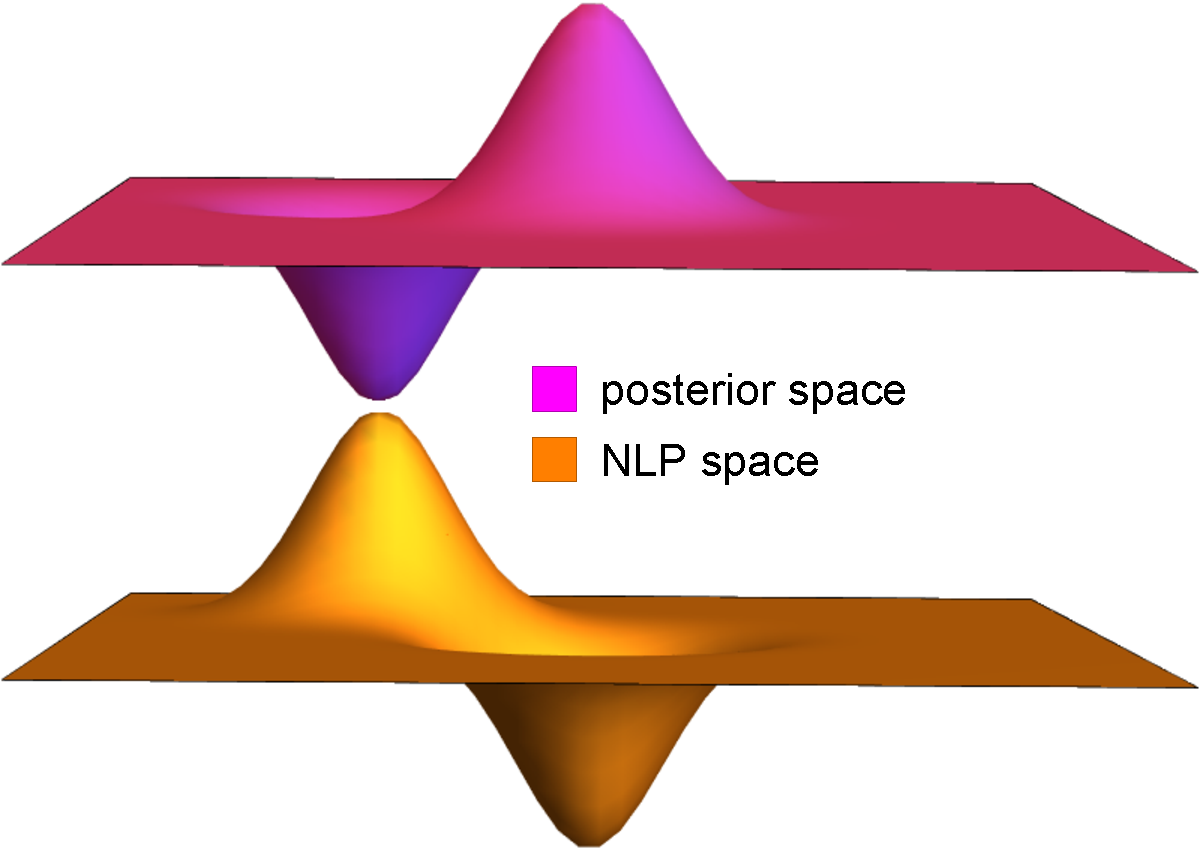
\includegraphics[width=1\textwidth]{./Figures/lec5_nlpPosterior1.pdf}}
	\end{figure}
	
\end{frame}

\begin{frame}
	\frametitle{Simulating the puck's motion in NLP space: consider a point in posterior space}
	
	\begin{figure}[ht]
		\centerline{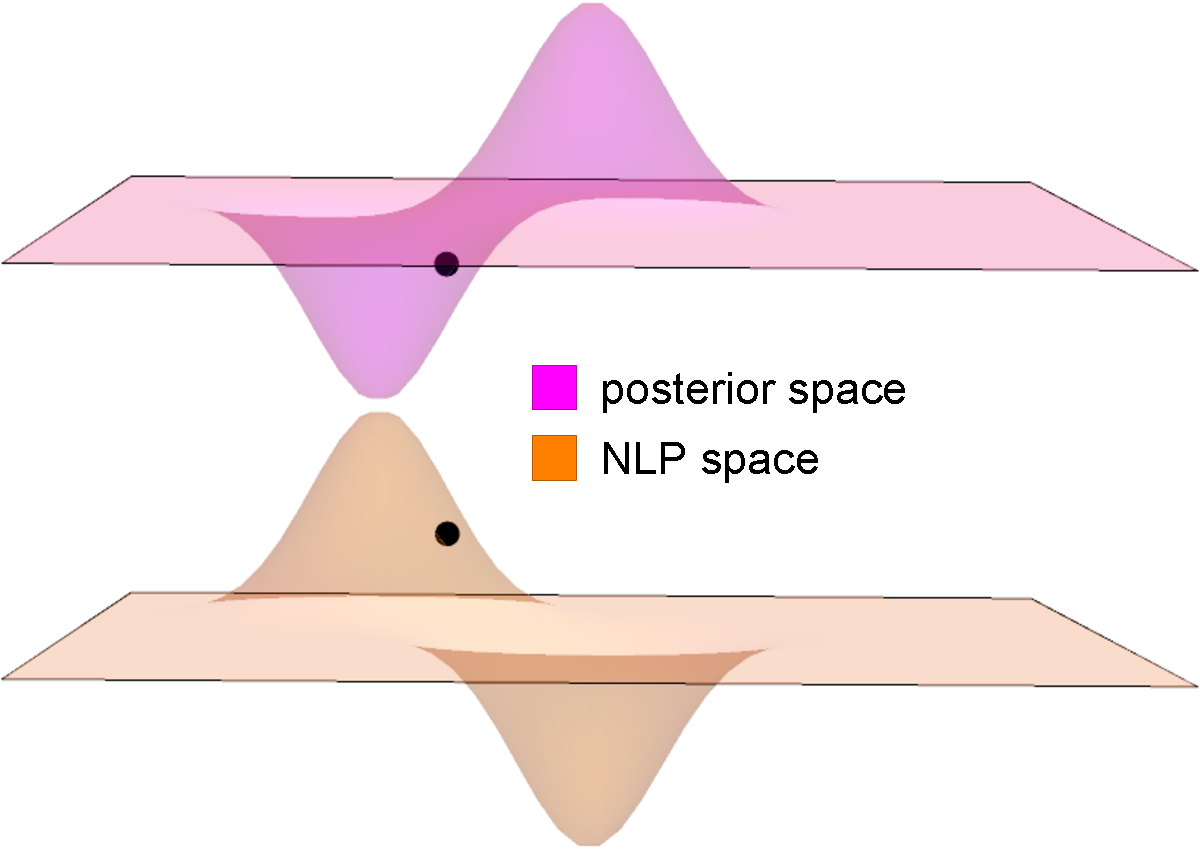
\includegraphics[width=1\textwidth]{./Figures/lec5_nlpPosterior2.pdf}}
	\end{figure}
	
\end{frame}

\begin{frame}
	\frametitle{The path traced out for 100 different shoves from same distribution}
	
	\begin{figure}[t]
		\centerline{\animategraphics[width=1\textwidth,controls,buttonsize=1em,buttonfg=0.5]{2}{./Animations/lec5_puckPath}{1}{26}}
	\end{figure}
	
\end{frame}

\begin{frame}
	\frametitle{The HMC algorithm}
	\onslide<2-> The HMC algorithm works as follows,
	
	\begin{itemize}
		\item<3-> Start at random location $\theta_0$.
		\item<4-> For $i=1,...,N$ do:
		\begin{enumerate}
			\item<5-> Give puck random initial momentum, $k\sim N(0,\Sigma)$.
			\item<6-> Simulate puck's movement across NLP surface for a fixed time $T$ (number of discrete steps of numerical integration algo).
			\item<7-> Compute a ratio:
			
			\begin{equation}
			r = \frac{p(\theta_t|X)}{p(\theta_{t-1}|X)} \times \frac{p(k')}{p(k)}
			\end{equation}
			
			where $k$ is the final momentum.
			
			\item<8-> If $r > u \implies$ move to $\theta_{t}$, otherwise return to $\theta_{t-1}$.
		\end{enumerate}
	\end{itemize}
	
\end{frame}

\begin{frame}
	\frametitle{The HMC algorithm}
	
	\begin{figure}[t]
		\centerline{\animategraphics[width=1\textwidth,controls,buttonsize=1em,buttonfg=0.5]{12}{./Animations/lec6_hmc_a}{1}{154}}
	\end{figure}
	
\end{frame}

\begin{frame}
	\frametitle{The HMC algorithm}
	
	\begin{figure}[t]
		\centerline{\animategraphics[width=1\textwidth,controls,buttonsize=1em,buttonfg=0.5]{12}{./Animations/lec6_hmc_b}{1}{154}}
	\end{figure}
	
\end{frame}

\begin{frame}
	\frametitle{The HMC algorithm}
	
	\begin{figure}[t]
		\centerline{\animategraphics[width=1\textwidth,controls,buttonsize=1em,buttonfg=0.5]{12}{./Animations/lec6_hmc_c}{1}{2}}
	\end{figure}
	
\end{frame}


\begin{frame}
	\frametitle{Simulating the puck's motion in NLP space: randomly shoving the puck at intervals of 50 steps}
	
	\begin{figure}[t]
		\centerline{\animategraphics[width=1\textwidth,controls,buttonsize=1em,buttonfg=0.5]{5}{./Animations/lec6_HMC}{1}{109}}
		\end{figure}
		
\end{frame}

\begin{frame}
	\frametitle{RWM and Gibbs performance}
	
	\begin{figure}[t]
		\centerline{\animategraphics[width=1\textwidth,controls,buttonsize=1em,buttonfg=0.5]{2}{./Animations/lec5_gibbsBirdsBothCorrelateda}{1}{30}}
	\end{figure}
	
\end{frame}

\begin{frame}
	\frametitle{Hamiltonian Monte Carlo performance}
	
	\begin{figure}[t]
		\centerline{\animategraphics[width=0.6\textwidth,controls,buttonsize=1em,buttonfg=0.5]{2}{./Animations/lec5_birdsHMC}{1}{30}}
	\end{figure}
	
\end{frame}

\begin{frame}
	\frametitle{Hamiltonian Monte Carlo: summary}
	
	\begin{itemize}
		\item<2-> Imagine a puck sliding across a frictionless surface of the negative log posterior (NLP).
		\item<3-> Give puck random shoves at predefined time intervals, and simulate path of puck for predefined time interval.
		\item<4-> Puck will tend to visit areas of low NLP which correspond to areas of high posterior density!
		\item<5-> Algorithm often performs considerably better than Random Walk Metropolis or Gibbs.
		\item<6-> Stan uses a fancy variant of HMC known as NUTS (No U-Turn Sampler) that determines the optimal time intervals to simulate puck for.
	\end{itemize}
	
\end{frame}


\section{Our first words in Stan}
\frame{\tableofcontents[currentsection]}

\begin{frame}
\frametitle{Coding up MCMC algorithms}
\begin{itemize}
\item<2-> Up until now we have coded up our own MCMC algorithms
$\implies$ (relatively) straightforward for simple models.
\item<3-> However for more complex models this is a time-consuming (and frustrating) process.
\item<4-> Flavours of MCMC algorithms:
\begin{itemize}
\item[-]<5-> \textbf{Random Walk Metropolis:} fairly basic but ineffectual for many real-life models.
\item[-]<6-> \textbf{Gibbs:} a bit faster than RWM but also suffers from same issues. However can be significantly harder to code up!
\item[-]<7-> \textbf{Hamiltonian Monte Carlo:} significantly more efficient than the aforementioned but also significantly harder to code and tune.
\end{itemize}
\end{itemize}


\end{frame}

\begin{frame}
\frametitle{Introducing Stan: avoiding manual labour}
\onslide<2->
\textbf{Stan} is an intuitive yet sophisticated programming language that does the hard work for us.

\onslide<3-> What is Stan and how do we use it?

\begin{itemize}
\item<4-> \textbf{Imperative} programming language like R, Python, Matlab, C++ etc. (BUGS/JAGS are a weird type of language called \textbf{declarative}.)
\item<5-> Turing-complete language (unlike BUGS/JAGS) and works like most other languages: can use loops, conditional statements, and functions.
\item<6-> Code up a model in Stan and then it implements Hamiltonian Monte Carlo (actually something called NUTS but similar) for us.
\end{itemize}

\end{frame}

\begin{frame}
\frametitle{Why should we use Stan?}

\begin{itemize}
\item<2-> Stan is the brainchild of Andrew Gelman at Colombia; the World's foremost Bayesian statistician.
\item<3-> Stan's uses an extension of HMC called NUTS that automatically tunes. It is \textbf{fast}. Very fast $\implies$ typically generates multiples times as many effective samples per second than BUGS/JAGS. 
\item<4-> Stan is \textbf{simple} to learn.
\item<5-> Stan has excellent documentation (a manual full of extensive examples).
\item<6-> The Stan team have translated \textbf{all} the example models from popular books; Gelman, Kruschke etc.
\item<7-> \textbf{Most important:} Stan has a very active and helpful user forum and development team; for example, typical question answered in less than a couple of hours.
\end{itemize}

\end{frame}

\begin{frame}
\frametitle{Why should we use Stan?}
\textbf{Overall:} Stan makes our life easier. 

\begin{itemize}
\item<2-> It is easy to learn; even if you are used to BUGS/JAGS or something else.
\item<3-> The language is here to stay $\implies$ all recent books use examples written in Stan rather than BUGS/JAGS.
\item<4-> \textbf{Important:} it is popular $\implies$ if you have a problem with your model you can get help, \textbf{fast}.
\item<5-> The best minds in the business are working on making it even better.
\item<6-> Finally, ``Shiny Stan'' makes it really quite fun!
\end{itemize}

\end{frame}

\begin{frame}
\frametitle{How do we use it?}

\begin{itemize}
\item<2-> Code up model in Stan code in a text editor and save as ``.stan'' file.
\item<3-> Call Stan to run the model from:
\begin{itemize}
\item[-]<4-> R.
\item[-]<5-> Python.
\item[-]<6-> The command line.
\item[-]<7-> Matlab.
\item[-]<8-> Stata.
\item[-]<9-> Julia.
\end{itemize}
\item<10-> Use one of the above to analyse the data (of course you can export to another one.)
\end{itemize}
\end{frame}

\begin{frame}
\frametitle{A straightforward example}
Suppose:
\begin{itemize}
\item<2-> We record the height, $Y_i$, of 10 people.
\item<3-> We want a model to explain the variation, and choose a normal likelihood:
\onslide<4-> 
\begin{equation}
Y_i \sim N(\mu,\sigma)
\end{equation}
\item<5-> We choose the following (independent) priors on each parameter:
\begin{itemize}
\item[-]<6-> $\mu\sim N(0,1)$.
\item[-]<7-> $\sigma\sim \text{gamma}(1,1)$.
\end{itemize}

\onslide<8->
\textbf{Question:} how do we code this up in Stan?
\end{itemize}

\end{frame}

\begin{frame}[fragile]
\frametitle{An example Stan program: heights}
	\begin{minted}{stan}
data {
    real Y[10]; // Heights for 10 people
}

parameters {
    real mu;
    real<lower=0> sigma;
}

model {
    Y ~ normal(mu,sigma); // Likelihood
    mu ~ normal(0,1); // Prior for mu
    sigma ~ gamma(1,1); // Prior for sigma
}
	\end{minted}

\end{frame}

\begin{frame}[fragile]
\frametitle{An example Stan program: data block}
\begin{minted}{stan}
data {
    real Y[10]; // Heights for 10 people
}
\end{minted}

\begin{itemize}
\item<2-> Declare all data that you will pass to Stan to estimate your model.
\item<3-> Terminate all statements with a semi-colon ``;''.
\item<4-> Use ``//'' for comments.
\end{itemize}

\end{frame}

\begin{frame}[fragile]
\frametitle{An example Stan program: data block}
\begin{minted}{stan}
data {
    real Y[10]; // Heights for 10 people
}
\end{minted}

\onslide<2-> Strongly, statically-typed language: need to tell Stan the type of data variable. For example:
\begin{itemize}
\item[-]<3-> \mintinline{stan}{real} for continuous data.
\item[-]<4-> \mintinline{stan}{int} for discrete data.
\item[-]<5-> Arrays: above we specified \mintinline{stan}{Y} as an array of continuous data of length 10.
\end{itemize}

\end{frame}

\begin{frame}[fragile]
\frametitle{An example Stan program: data block}
\begin{minted}{stan}
data {
    real Y[10]; // Heights for 10 people
}
\end{minted}

\begin{itemize}
\item<2-> Can place limits on data, for example:
\begin{itemize}
	\item[-]<3-> \mintinline{stan}{real<lower=0,upper=1> X}
	\item[-]<4-> \mintinline{stan}{real<lower=0> Z}
\end{itemize}
\item<5-> Vectors and matrices; only contain reals and can be used for matrix operations. 
\end{itemize}

\end{frame}

\begin{frame}[fragile]
\frametitle{An example Stan program: parameter block}
\begin{minted}{stan}
parameters {
    real mu;
    real<lower=0> sigma;
}
\end{minted}
\begin{itemize}
\item<2-> Declare all parameters that you use in your model.
\item<3-> Place limits on variables, for example  \mintinline{stan}{real<lower=0> sigma} above.
\item<4-> A multitude of parameter types including some of the aforementioned:
\begin{itemize}
\item[-]<5-> \mintinline{stan}{real} for continuous parameters.
\item[-]<6-> Arrays of types, for example \mintinline{stan}{real epsilon[12]}.
\end{itemize}
\end{itemize}

\end{frame}

\begin{frame}[fragile]
\frametitle{An example Stan program: parameter block}
\begin{minted}{stan}
parameters {
    real mu;
    real<lower=0> sigma;
}
\end{minted}
\begin{itemize}
\item<2-> \mintinline{stan}{vector} or \mintinline{stan}{matrix}, specified by:
\begin{itemize}
	\item[-]<3-> \mintinline{stan}{vector[5] beta}
	\item[-]<4-> \mintinline{stan}{matrix[5,3] gamma}
\end{itemize}
\item<5-> \mintinline{stan}{simplex} for a parameter vector that must sum to 1.
\item<6-> More exotic types like \mintinline{stan}{corr_matrix} , or \mintinline{stan}{ordered}.
\end{itemize}

\end{frame}

\begin{frame}[fragile]
\frametitle{An example Stan program: parameter block}
\begin{minted}{stan}
parameters {
    real mu;
    real<lower=0> sigma;
}
\end{minted}
\onslide<2->
\textbf{Important:} HMC/NUTS not developed yet to work with \textbf{discrete} parameters $\implies$ following options in Stan:

\begin{itemize}
\item<3-> Marginalise out the parameter. For example, if $p(\beta,\theta)$ where $\beta$ is continuous and $\theta$ is discrete:
\onslide<4->
\begin{equation}
p(\beta) = \sum\limits_{i=1}^{K} p(\beta,\theta_i)
\end{equation}
\item<5-> Some models can be reformulated without discrete parameters.
\item<6-> Failing either of the above $\implies$ use BUGS/JAGS.
\end{itemize}

\end{frame}

\begin{frame}[fragile]
\frametitle{An example Stan program: model block}
\begin{minted}{stan}
model {
    Y ~ normal(mu,sigma); // Likelihood
    mu ~ normal(0,1); // Prior for mu
    sigma ~ gamma(1,1); // Prior for sigma
}
\end{minted}
\begin{itemize}
\item<2-> Used to define:
\begin{itemize}
\item[-]<3-> Likelihood.
\item[-]<4-> Priors on parameters.
\end{itemize}
\item<5-> If don't specify priors on parameters $\implies$ Stan assumes you are using flat priors (which can be improper.)
\end{itemize}

\end{frame}

\begin{frame}[fragile]
\frametitle{An example Stan program: model block}
\begin{minted}{stan}
model {
    Y ~ normal(mu,sigma); // Likelihood
    mu ~ normal(0,1); // Prior for mu
    sigma ~ gamma(1,1); // Prior for sigma
}
\end{minted}
\begin{itemize}
\item<2-> \textbf{Huge} range of probability distributions covered, across a range of parameterisations. For example: 
\begin{itemize}
\item[-]<3-> \textbf{Discrete:} Bernoulli, binomial,  normal, poisson, beta-binomial, negative-binomial, categorical, multinomial.
\item[-]<4-> \textbf{Continuous unbounded:} normal, skew-normal, Student-t, Cauchy, logistic.
\item[-]<5-> \textbf{Continuous bounded:} uniform, beta, log-normal, exponential, gamma, Chi-squared, inverse-Chi-squared, Weibull, Wiener diffusion, Pareto. 
\end{itemize}
\end{itemize}
\end{frame}

\begin{frame}[fragile]
\frametitle{An example Stan program: model block}
\begin{minted}{stan}
model {
    Y ~ normal(mu,sigma); // Likelihood
    mu ~ normal(0,1); // Prior for mu
    sigma ~ gamma(1,1); // Prior for sigma
}
\end{minted}
\begin{itemize}
\item[-]<2-> \textbf{Multivariate continuous:} normal, Student-t, gaussian process.
\item[-]<3-> \textbf{Exotics:} Dirichlet, LKJ correlation distribution, Wishart and its inverse, Von-Mises.
\end{itemize}
\end{frame}

\begin{frame}
\frametitle{Running Stan}

\onslide<2-> Write model in a text editing program. For example:
\begin{itemize}
\item 3-> \textbf{RStudio} -- offers Stan syntax highlighting.
\item<3-> \textbf{emacs} - Stan syntax actually supported.
\item<4-> \textbf{notepad++}.
\end{itemize}

\onslide<6-> $\implies$ save as ``exampleModel.stan'' in same directory as you run statistical software.



\end{frame}

\begin{frame}[fragile]
	\frametitle{Running Stan in R}
	\begin{knitrout}\footnotesize
		\definecolor{shadecolor}{rgb}{0.969, 0.969, 0.969}\color{fgcolor}\begin{kframe}
			\begin{alltt}
				\hlcom{## Load packages}
				\hlkwd{library}\hlstd{(rstan)}
			\end{alltt}
\begin{alltt}
				\hlcom{## Generate fake data}
				\hlstd{Y} \hlkwb{=} \hlkwd{rnorm}\hlstd{(}\hlnum{10}\hlstd{,}\hlkwc{mean} \hlstd{=} \hlnum{0}\hlstd{,} \hlkwc{sd} \hlstd{=} \hlnum{1}\hlstd{)}
				
				\hlcom{## Compile and run model, and save in fit}
				\hlstd{fit} \hlkwb{=} \hlkwd{stan}\hlstd{(}\hlkwc{file}\hlstd{=}\hlstr{'exampleModel.stan'}\hlstd{,}\hlkwc{data}\hlstd{=}\hlkwd{list}\hlstd{(}\hlkwc{Y}\hlstd{=Y),}
				            \hlkwc{iter}\hlstd{=}\hlnum{1000}\hlstd{,}\hlkwc{chains}\hlstd{=}\hlnum{4}\hlstd{)}
			\end{alltt}
		\end{kframe}
	\end{knitrout}
\end{frame}

\begin{frame}[fragile]
\frametitle{Running Stan on example model}
\begin{knitrout}\footnotesize
	\definecolor{shadecolor}{rgb}{0.969, 0.969, 0.969}\color{fgcolor}\begin{kframe}
		\begin{alltt}
			\hlcom{## Compile and run model, and save in fit}
			\hlstd{fit} \hlkwb{=} \hlkwd{stan}\hlstd{(}\hlkwc{file}\hlstd{=}\hlstr{'exampleModel.stan'}\hlstd{,}\hlkwc{data}\hlstd{=}\hlkwd{list}\hlstd{(}\hlkwc{Y}\hlstd{=Y),}
			            \hlkwc{iter}\hlstd{=}\hlnum{1000}\hlstd{,}\hlkwc{chains}\hlstd{=}\hlnum{4}\hlstd{)}
		\end{alltt}
	\end{kframe}
\end{knitrout}

\onslide<2->
The above R code runs NUTS for our model with the following options:
\begin{itemize}
\item<3-> 1000 MCMC samples of which 500 are discarded as warm-up.
\item<4-> Across 4 chains.
\item<5-> Using a random number seed of 1 (good to ensure you can reproduce results.)
\end{itemize}

\end{frame}

\begin{frame}[fragile]
\frametitle{Example model: results}
	\begin{knitrout}\small
		\definecolor{shadecolor}{rgb}{0.969, 0.969, 0.969}\color{fgcolor}\begin{kframe}
			\begin{alltt}
				\hlcom{## Print summary statistics}
				\hlkwd{print}\hlstd{(fit,}\hlkwc{probs} \hlstd{=} \hlkwd{c}\hlstd{(}\hlnum{0.25}\hlstd{,} \hlnum{0.5}\hlstd{,} \hlnum{0.75}\hlstd{))}
			\end{alltt}
			\begin{verbatim}
			## Inference for Stan model: exampleModel.
			## 4 chains, each with iter=1000; warmup=500; thin=1; 
			## post-warmup draws per chain=500
			## 
			##        mean se_mean   sd   25%   50%   75% n_eff Rhat
			## mu    -0.02    0.01 0.28 -0.20 -0.02  0.16   689    1
			## sigma  0.95    0.01 0.24  0.78  0.91  1.08   696    1
			## lp__  -5.26    0.04 1.00 -5.69 -4.97 -4.50   639    1
			\end{verbatim}
		\end{kframe}
	\end{knitrout}
\end{frame}

\begin{frame}[fragile]
\frametitle{Example model: results}
	\begin{knitrout}\small
		\definecolor{shadecolor}{rgb}{0.969, 0.969, 0.969}\color{fgcolor}\begin{kframe}
			\begin{alltt}
				\hlcom{## Extract element and plot}
				\hlstd{mu} \hlkwb{=} \hlkwd{extract}\hlstd{(fit,}\hlstr{'mu'}\hlstd{)[[}\hlnum{1}\hlstd{]]}
				
				\hlcom{## Plot histogram}
				\hlkwd{library}\hlstd{(ggplot2)}
				\hlkwd{qplot}\hlstd{(mu,} \hlkwc{fill}\hlstd{=}\hlkwd{I}\hlstd{(}\hlstr{"blue"}\hlstd{))}
			\end{alltt}
\end{kframe}
		
		
	\end{knitrout}
	
	\begin{figure}[ht]
		\centerline{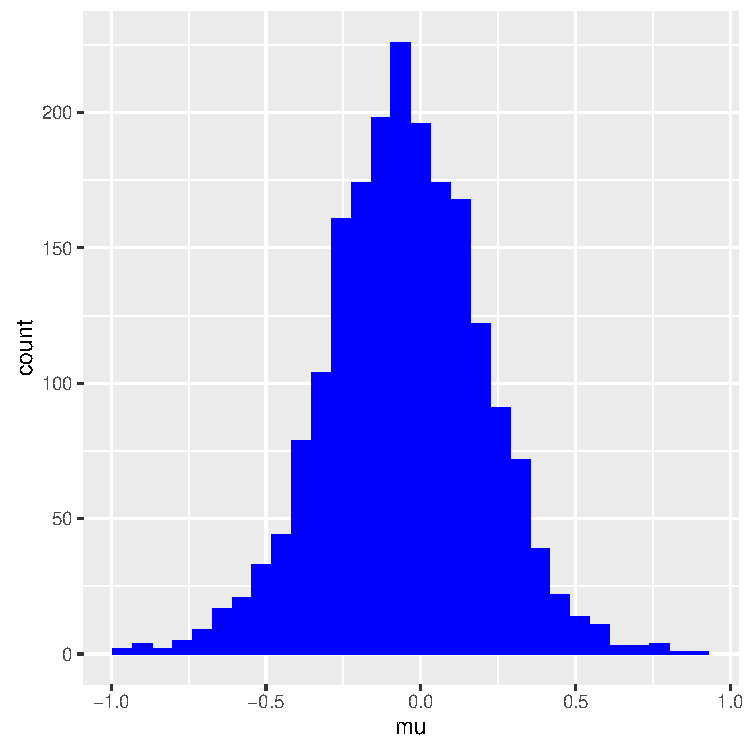
\includegraphics[width=.4\linewidth]{./Figures/boring-plots1-1.pdf} }
	\end{figure}
	
\end{frame}

\begin{frame}
	\frametitle{Example model: results}
\begin{figure}[ht]
	\centerline{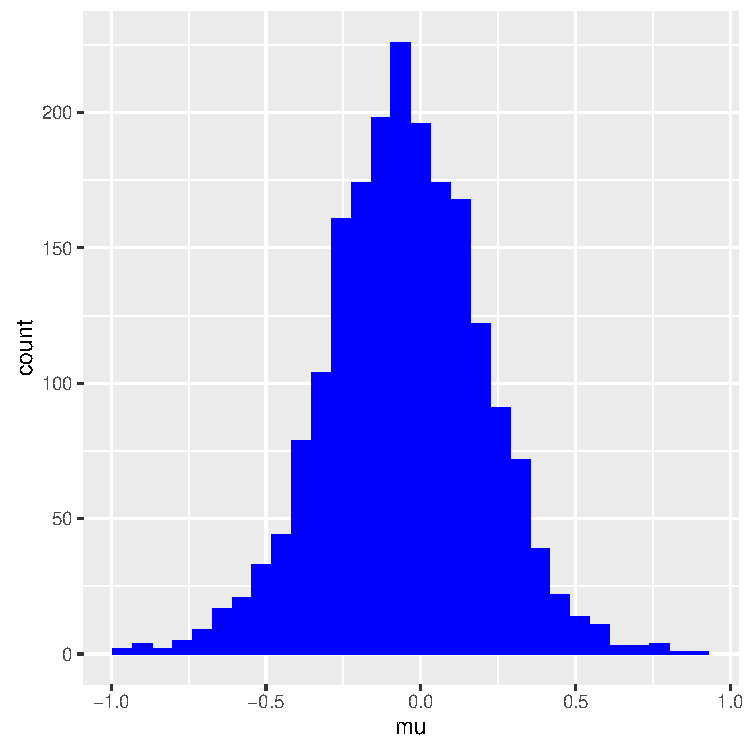
\includegraphics[width=0.75\textwidth]{./Figures/boring-plots1-1.pdf}}
\end{figure}
\end{frame}

\begin{frame}[fragile]
	\frametitle{Quick note: what does $\sim$ actually mean?}
	\begin{minted}{stan}
model {
    Y ~ normal(mu,sigma); // Likelihood
    mu ~ normal(0,1); // Prior for mu
    sigma ~ gamma(1,1); // Prior for sigma
}
	\end{minted}
	\begin{itemize}
		\item<2-> $\sim$ doesn't mean ``sampling'' although for many circumstances it isn't terrible to think of it like that.
		\item<3-> Remember: HMC/NUTS uses the negative of the log-posterior to find potential energy of puck.
		\item<4-> $\implies$ logging the posterior converts it from a product into a sum.
		\item<5-> As such $\sim$ really means ``increment log probability''.
	\end{itemize}
	
\end{frame}

\begin{frame}
	\frametitle{Sleep deprivation study: revisited}
	\begin{itemize}
		\item<2-> Data from a laboratory experiment that measured the effect of sleep deprivation on cognitive performance \footcite{belenky2003patterns}.
		\item<3-> 18 subjects within a population of interest - long-distance lorry drivers - volunteered to participate in the 10 day experiment.
		\item<4-> Subjects were restricted to 3 hours of sleep per night.
		\item<5-> On each day the subjects' reaction time across a range of cognitive tasks were measured.
	\end{itemize}
	
	\begin{figure}[ht]
		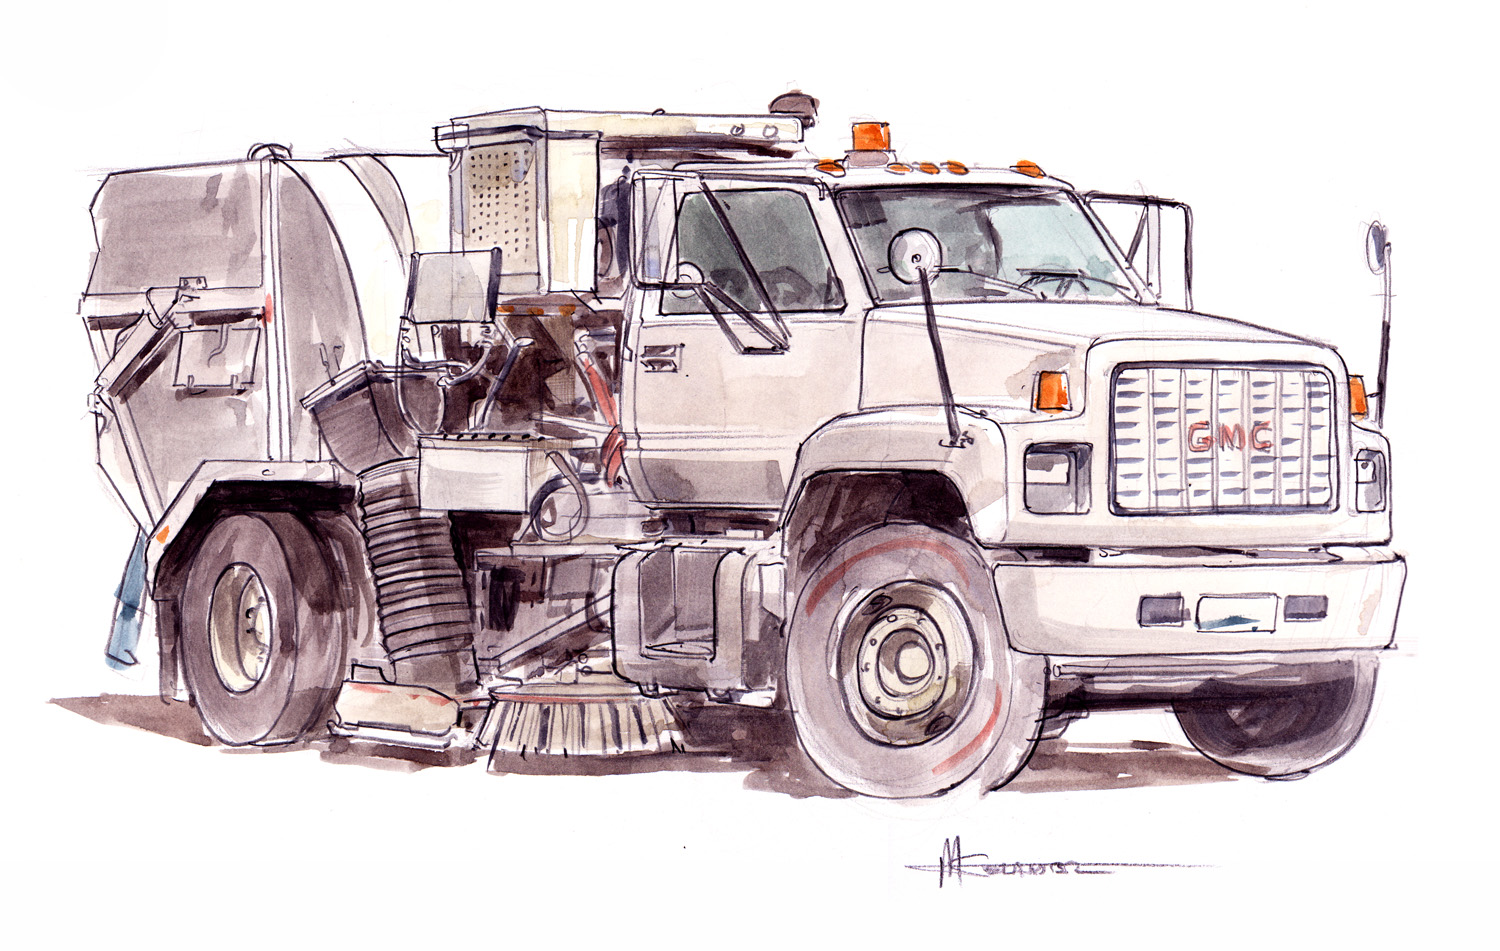
\includegraphics[width=1.0\textwidth]{./Figures/lorry.jpg}
	\end{figure}
	
\end{frame}

\begin{frame}
	\frametitle{Sleep deprivation study: model aims}
	
	\begin{itemize}
		\item<2-> Build a model to explain the effect of sleep deprivation on reaction times.
	\end{itemize}
	
	\onslide<3->
	\begin{figure}[ht]
		\centerline{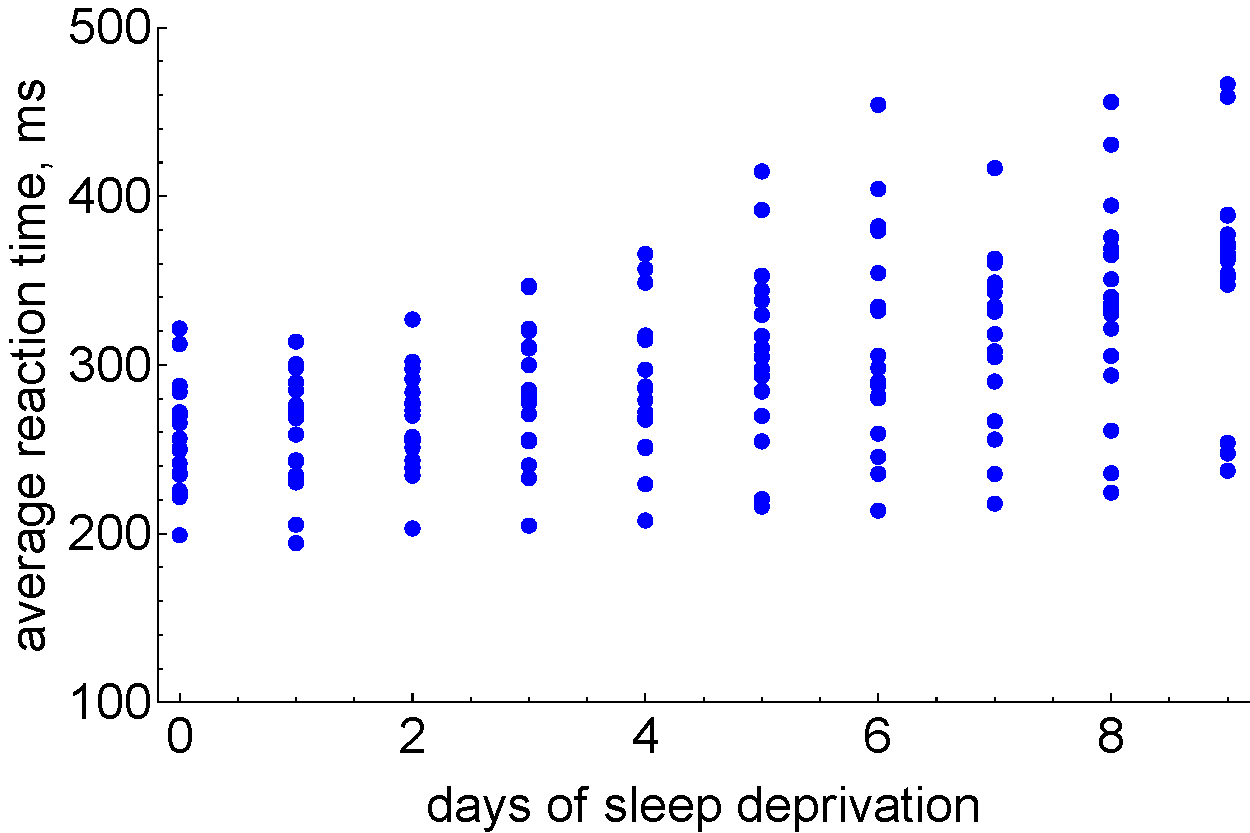
\includegraphics[width=0.9\textwidth]{./Figures/lec4_sleepData.pdf}}
	\end{figure}
	
\end{frame}

\begin{frame}
	\frametitle{Sleep deprivation study: model}
	\onslide<2-> On the basis of the previous graph, assume:
	
	\onslide<3->
	\begin{equation}
	R(t)\sim N(\alpha + \beta t,\sigma)
	\end{equation}
	
	\onslide<4-> where $R(t)$ is the reaction time for a sleep deprivation of $t$ days. 
	
	\onslide<5-> \textbf{Question:} how can we code this up in Stan?
	
	\onslide<1->
	\begin{figure}[ht]
		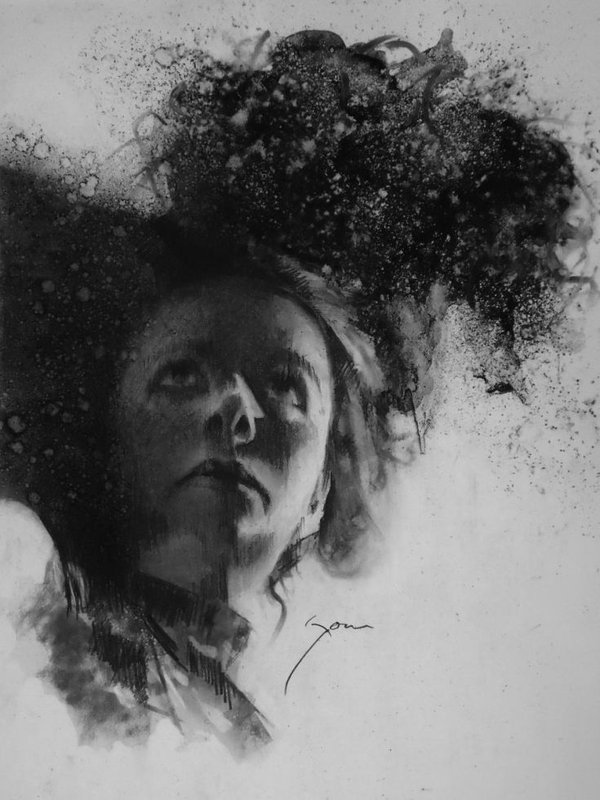
\includegraphics[width=0.7\textwidth]{./Figures/sleep.jpg}
	\end{figure}
	
\end{frame}

\begin{frame}[fragile]
	\frametitle{Sleep deprivation study: 1st part of Stan code}
\begin{minted}{stan}
data {
    int N; // number of observations
    vector[N] t; // days of sleep deprivation
    vector[N] R; // reaction times
} 
parameters {
    real alpha; // reaction time at start
    real beta; // daily increment to reaction time
    real<lower=0> sigma; // variation about mean
} 
\end{minted}
	
\end{frame}

\begin{frame}[fragile]
	\frametitle{Sleep deprivation study: 2nd part of Stan code}
	\begin{minted}{stan}
model {
    // likelihood
    for (i in 1:N){
        R[i] ~ normal(alpha + beta * t[i], sigma);
    }
    
    // priors
    alpha ~ normal(0,250);
    beta ~ normal(0,250);
    sigma ~ normal(0,50);
}
	\end{minted}
	
\end{frame}

\begin{frame}[fragile]
	\frametitle{Sleep deprivation study: 2nd part of Stan code}
    However can write same model with faster and more efficient Stan code using vectorization.
    
   	\begin{minted}{stan}
data {
    int N; // number of observations
    matrix[N,2] X; // ones + days of sleep depriv.
    vector[N] R; // reaction times
 } 
 parameters {
    vector[2] gamma;
    real<lower=0> sigma;
  } 
model {
     // likelihood
     R ~ normal(X * gamma, sigma);
     gamma ~ normal(0,250);
}
  	\end{minted}
    
\end{frame}

\begin{frame}[fragile]
	\frametitle{Sleep deprivation study: posterior predictive distribution}
	\begin{itemize}
		\item<2-> Want to carry out posterior predictive checks $\implies$ need posterior predictive distribution.
		\item<3-> Use ``generated quantities'' block.
	\end{itemize}

\onslide<4->
\begin{minted}{stan}
generated quantities {
    vector[N] R_sim; // Store post-pred samples
    for (i in 1:N){
        R_sim[i] = normal_rng(X[i] * gamma, sigma);
    }
}
\end{minted}
	
\end{frame}

\begin{frame}[fragile]
	\frametitle{Sleep deprivation study: posterior predictive distribution}
    \begin{minted}{stan}
generated quantities {
	vector[N] R_sim; // Store post-pred samples
	for (i in 1:N){
        R_sim[i] = normal_rng(X[i] * gamma, sigma);
    }
}
	\end{minted}
	
\onslide<2-> The function \mintinline{stan}{normal_rng} generates a single \textbf{independent} sample from a normal distribution with parameters:

\begin{itemize}
	\item<3-> $\text{mean} = X[i] * gamma$, where $gamma$ is a sample from the estimated posterior.
	\item<4-> $\text{std. dev} = sigma$, where $sigma$ is a sample from the estimated posterior. 
\end{itemize}
\end{frame}

\begin{frame}[fragile]
	\frametitle{Sleep deprivation study: model changes}
	\begin{itemize}
		\item<2-> Suppose based on posterior predictive checks we want to use a wider sampling distribution $\implies$ use a Student T.
		\item<3-> If we were coding this up ourselves this would involve a large structural change in the code and MCMC algorithm.
	\end{itemize}
	
	\onslide<4->\textbf{Question:} how long does it take us to recode our model in Stan?
	

\end{frame}

\begin{frame}[fragile]
	\frametitle{Sleep deprivation study: model changes}
	\begin{minted}{stan}
parameters {
    ...
    real<lower=0> nu;
} 
model {
    // likelihood
    R ~ student_t(nu, X * gamma, sigma);
    ...
    nu ~ gamma(1,1);
}
	\end{minted}
\onslide<2-> $\implies$ three changes/additions necessary.
	
\end{frame}

\begin{frame}
	\frametitle{Sleep deprivation: posterior predictive checks}
	Posterior predictive distribution for Student T sampling.
	
	\begin{figure}[ht]
		\centerline{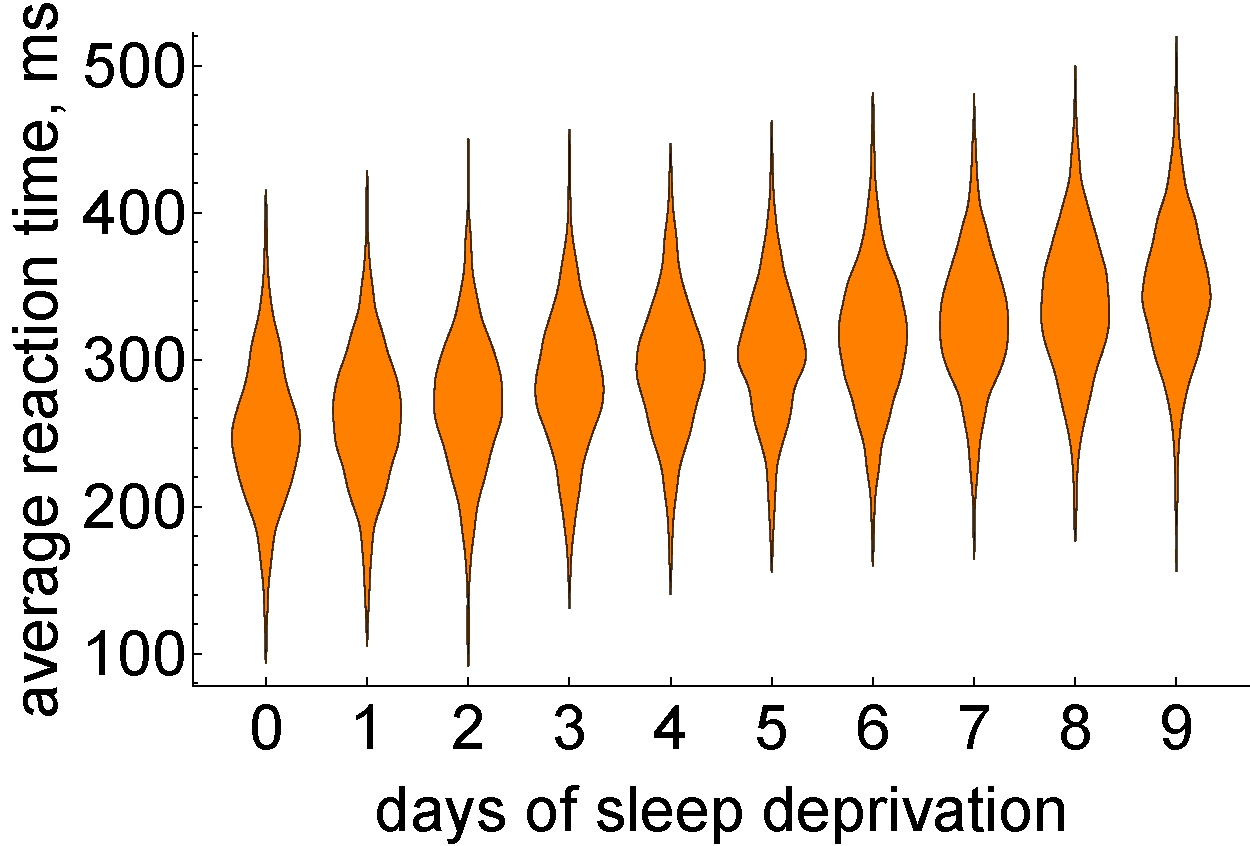
\includegraphics[width=1\textwidth]{./Figures/lec6_sleepPPC1.pdf}}
	\end{figure}
	
\end{frame}

\begin{frame}
	\frametitle{Sleep deprivation: posterior predictive checks}
	One participant.
	
	\begin{figure}[ht]
		\centerline{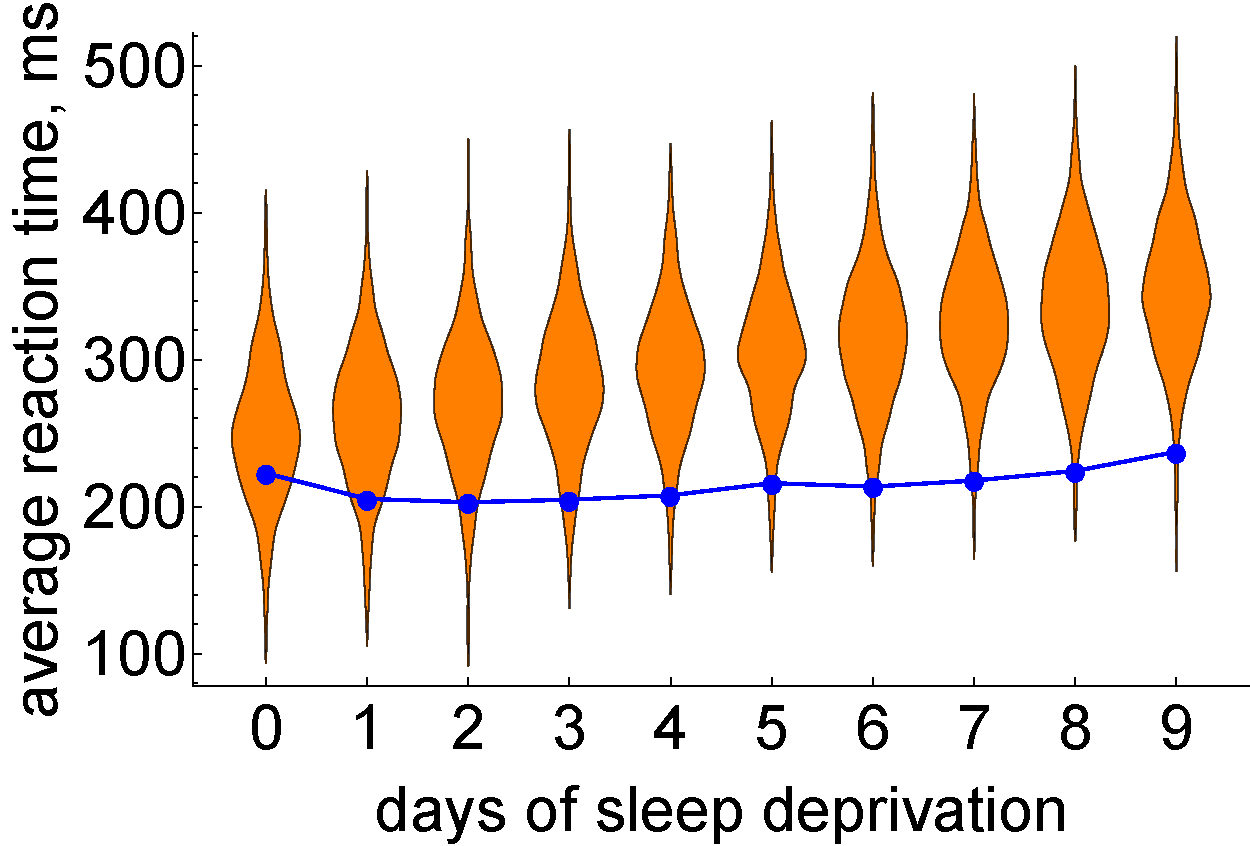
\includegraphics[width=1\textwidth]{./Figures/lec6_sleepPPC2.pdf}}
	\end{figure}
	
\end{frame}

\begin{frame}
	\frametitle{Sleep deprivation: posterior predictive checks}
	And another.
	
	\begin{figure}[ht]
		\centerline{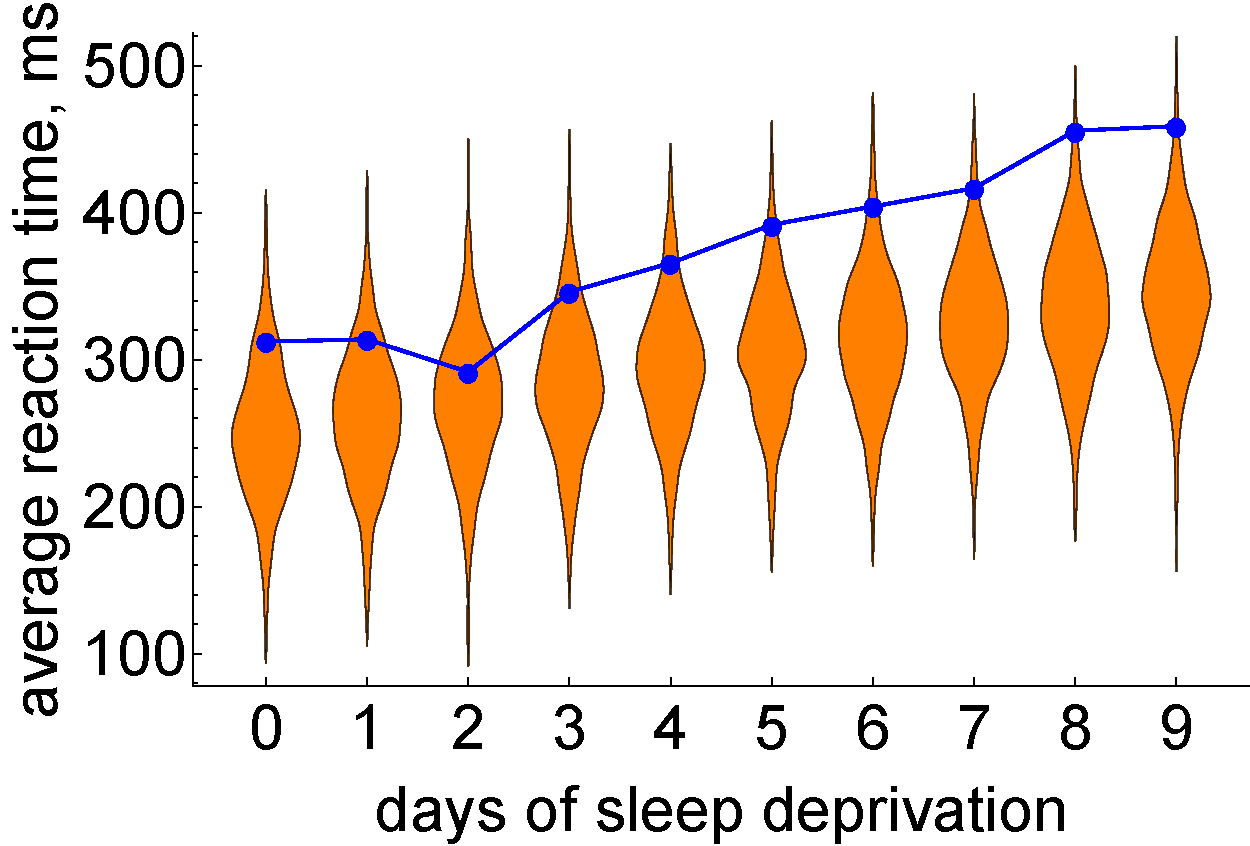
\includegraphics[width=1\textwidth]{./Figures/lec6_sleepPPC3.pdf}}
	\end{figure}
	
\end{frame}

\begin{frame}
	\frametitle{Sleep deprivation study: model changes}
	\onslide<2-> Moving to a Student T distribution did not solve individual fit issues $\implies$ try a more ambitious change:
	
	\begin{itemize}
		\item<3-> Go back to normal sampling model.
		\item<4-> Allow each subject their own response parameters.
		\item<5-> $\implies$ parameters are now 18-dimensional; one per each of the 18 subjects.
		\item<6-> (A better way to do this is with hierarchical models; more on this later.)
	\end{itemize}
	
	\vspace{0.2cm}
	
	\onslide<7-> 
	\textbf{Question:} how long does this modification take us?

	
\end{frame}

\begin{frame}[fragile]
	\frametitle{Sleep deprivation study: model changes}
		\begin{minted}{stan}
data {
    ...
    ## array of subject ids: 1, 2,..,18
    int subject[N];
}
parameters {
    ...
    real alpha[18]; ## 18 elements of each param
    real beta[18]; ## one for each subject
} 
model {
    for (i in 1:N){
        R[i] ~ normal(alpha[subject[i]] + 
                  beta[subject[i]] * t[i], sigma);
    }
}
\end{minted}
\end{frame}

\begin{frame}
	\frametitle{Sleep deprivation: posterior predictive checks}
	First problematic subject.
	
	\begin{figure}[ht]
		\centerline{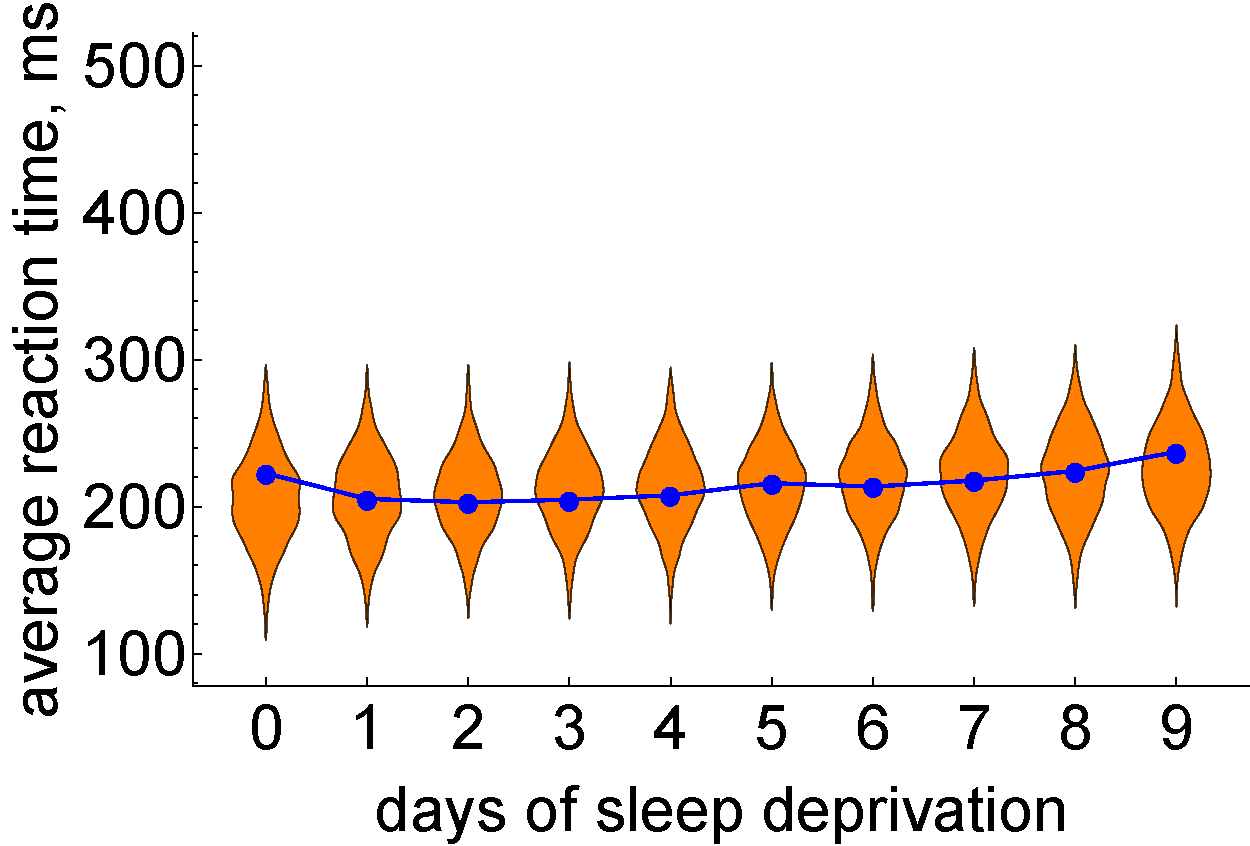
\includegraphics[width=1\textwidth]{./Figures/lec6_sleepPPCHeterogeneous1.pdf}}
	\end{figure}
	
\end{frame}

\begin{frame}
	\frametitle{Sleep deprivation: posterior predictive checks}
	Other problematic subject.
	
	\begin{figure}[ht]
		\centerline{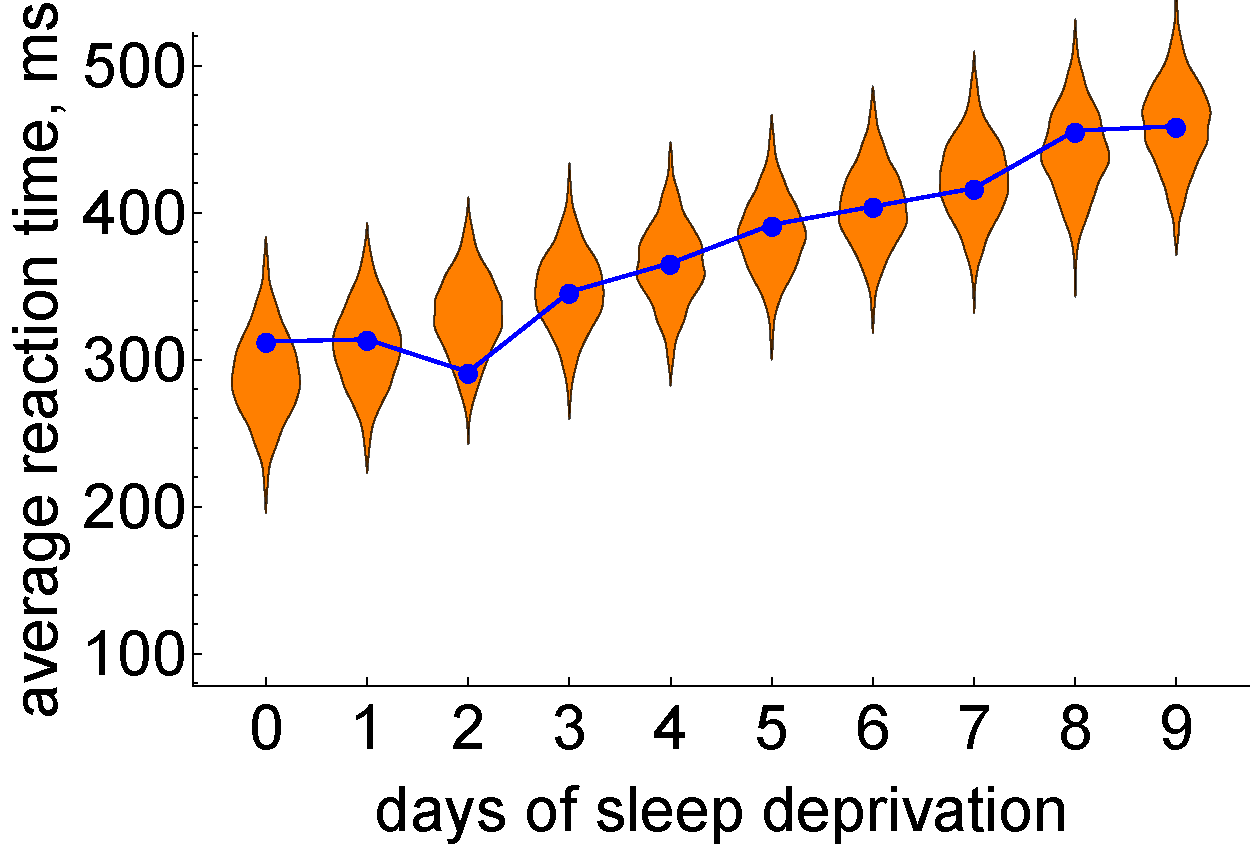
\includegraphics[width=1\textwidth]{./Figures/lec6_sleepPPCHeterogeneous2.pdf}}
	\end{figure}
	
\end{frame}

\begin{frame}[fragile]
\frametitle{Stan: a few of the loops and conditions}
\onslide<2-> Stan has pretty much the full range of language constructs to allow pretty much any model to be coded.
\onslide<3->
\begin{minted}{stan}
    for (i in 1:10) {something;}
    
    while (i > 1) {something;}

    if(i > 1) {something 1;}
    else if (i==0) {something2;}
    else {something 3;}
\end{minted}

\onslide<4-> \textbf{Note:} this is not the case with JAGS/BUGS due to their \textbf{declarative} nature.
	
\end{frame}

\begin{frame}
	\frametitle{Stan: speed concerns}
	\onslide<2-> Whilst Stan is fast it pays to know the importance of each code block for efficiency.
	
	\begin{itemize}
		\item<3-> \textbf{data} - called once at beginning of execution.
		\item<4-> \textbf{parameters} - every log probability evaluation!
		\item<5-> \textbf{model} - every log probability evaluation!
		\item<6-> \textbf{generated quantities} - once per sample.
	\end{itemize}	
	
\end{frame}

\begin{frame}
	\frametitle{Remaining code blocks}
	\onslide<2-> Thus far focussed on the four main code blocks, but others exist:
	
	\begin{itemize}
		\item<3-> \textbf{transformed data} - carry out a data transformation in Stan; executed once after data.
		\item<4-> \textbf{transformed parameters} - often easier to work with transformations of original parameters; executed every log probability evaluation!
		\item<5-> \textbf{functions} - allows user-defined functions, must go at top of Stan program. How many times it is called depends on the function's nature. Make it possible to use any density whose log pdf can be written down (see problem set)!
	\end{itemize}
\end{frame}

\begin{frame}[fragile]
	\frametitle{Stan in parallel}
	\onslide<2-> In R can run chains in parallel easily using:
	
	\onslide<3-> 
	\begin{kframe}
	\begin{alltt}
		\hlcom{# smaller font size for chunks}
		\hlkwd{library}\hlstd{(rstan)}
		\hlkwd{options}\hlstd{(}\hlkwc{mc.cores}\hlstd{=}\hlnum{8}\hlstd{)}
	\end{alltt}
\end{kframe}
\end{frame}

\begin{frame}
	\frametitle{Stan summary}
	
	\begin{itemize}
		\item<2-> Stan works by default with a HMC-like algorithm called NUTS.
		\item<3-> The Stan language is similar in nature to other common languages  with loops, conditional statements and user-definable functions (didn't cover here).
		\item<4-> Stan makes life easier for us than coding up the MCMC algorithms ourselves.
		\item<5-> Stan is typically multiple-times faster than BUGS/JAGS for generating effective samples.
	\end{itemize}
	
\end{frame}


\section{What to do when things go wrong}
\frame{\tableofcontents[currentsection]}

\begin{frame}
	\frametitle{How to debug a Stan model?}
	\onslide<2-> Two issue flavours, each with their own response.
	
	\begin{itemize}
		\item<2-> Coding errors.
		\item<3-> Sampling issues.
	\end{itemize}
	
\end{frame}

\begin{frame}[fragile]
	\frametitle{Coding errors}
	\onslide<2-> Stan error messages are generally quite informative however inevitably there are times when it is less clear why code fails
	
	\onslide<3-> $\implies$ debug by print!

\onslide<4->	
\begin{minted}{stan}
model {
    ...
    print(theta);
}
\end{minted}

\onslide<5-> In R this prints (neatly) to the console output.
	
\end{frame}

\begin{frame}
	\frametitle{Coding errors}
	\onslide<2->
	\textbf{Important:} failing a resolution via the above go to \url{http://mc-stan.org/} and do:
	
	\begin{enumerate}
		\item<3-> Look through manual for a solution.
		\item<4-> Look through user forum for previous answers to similar problems.
		\item<5-> Ask a question; be clear, and thorough - post as simple a model that replicates the issue.
		\item<6-> Ask me!
	\end{enumerate}
	
\end{frame}

\begin{frame}
\frametitle{Sampling issues}
\onslide<2-> Different sort of issue to a coding error, and falls into two (often related) issues:

\begin{itemize}
	\item<3-> \textbf{Slow convergence:} still have $\hat{R}>1.1$ after many thousands of iterations.
	\item<4-> \textbf{Divergent iterations:} get a warning in output from Stan with the number of iterations where the NUTS sampler has terminated prematurely.
\end{itemize}

\end{frame}

\begin{frame}
	\frametitle{Sampling issues}
	\onslide<2->
	\textbf{Most important thing today:} Gelman's ``Folk Theorem'':
	
	\vspace{0.2cm}
	
	\onslide<3-> 
	``Issues with computational sampling are almost always due to problems with the underlying statistical model, \textbf{not} the algorithm.''
	
\end{frame}

\begin{frame}
	\frametitle{Sampling issues: slow convergence}
    \begin{itemize}
    	\item<2-> Poor chain mixing is usually due to lack of \textbf{parameter identification}.
    	\item<3-> A parameter is identified if it has some unique effect on the data generating process that can be separated from the effect of the other parameters.
    \end{itemize}
    
    \onslide<4->
    \textbf{Solution (very important):} use \textbf{fake data} where you know the true parameter values.
    
    \vspace{0.2cm}
    
    \onslide<5->
    $\implies$ informative as to whether the data + priors are sufficient to estimate a parameter's value.
    
    \onslide<6-> If possible use the most simple version of your model that replicates the error.
    
\end{frame}

\begin{frame}
	\frametitle{Sampling issues: slow convergence}
	\onslide<2-> A significant number of divergent transitions of NUTS are problematic:
	\begin{itemize}
		\item<3-> Indicates that the stepwise integrator used to approximate Hamiltonian dynamics has likely diverged from exact trajectory.
		\item<4-> Therefore these samples \textbf{cannot} be viewed as being from the posterior.
		\item<5-> Causes a bias away from problem area of parameter space.
		\item<6-> Almost always because the step size is too large relative to the curvature of the posterior.
		\item<7-> However can be due to placing limits on parameters that preclude an area of high probability mass. 
	\end{itemize}
	
	\onslide<8->
	\textbf{Diagnosing problem:} use Shiny Stan (or otherwise) to make pairwise plots of variables $\implies$ look for parameters with high bivariate correlation; indicates high curvature.

\end{frame}

\begin{frame}
	\frametitle{Sampling issues: slow convergence}
	
	\onslide<2->
	\textbf{Solution:} if significant number of divergent iterations do the following:
	\begin{enumerate}
		\item<3-> Lower step size and increase acceptance rate in the call to Stan from R or otherwise.
		\item<4-> If above doesn't help change priors then likelihood.
	\end{enumerate}
	
	\onslide<5->
	Again failing all the above look at the Stan user forums, then ask a question.
	
\end{frame}

\begin{frame}
	\frametitle{What to do when things go wrong: summary}
	
	\begin{itemize}
		\item<2-> To debug a model that fails read error messages carefully, then try ``print'' statements.
		\item<3-> Problems with sampling are almost invariably problems with the underlying model \textbf{not} the sampling algorithm per se.
		\item<4-> Use fake data with all models to test for parameter identification (and that you've coded up correctly.)
		\item<5-> Stan has an active developer and user forum, great documentation, and an extensive answer bank.
		\item<6-> If you ask a question on the forum include your model, or ideally a simplified version that replicates the issue.
	\end{itemize}
	
\end{frame}

\begin{frame}
	\frametitle{Lecture summary}
	\begin{itemize}
		\item<2-> Hamiltonian Monte Carlo lets posterior geometry determine proposals by simulating movement of a puck in NLP space $\implies$ get high proportion of acceptances, and fast exploration of posterior space.
		\item<3-> Stan carries out inference by a variant of HMC called NUTS $\implies$ very fast!
		\item<4-> Stan is (hopefully) a fairly intuitive language to learn.
		\item<5-> Makes MCMC sampling easier for a wide class of problems in Bayesian inference.
		\item<6-> If things go wrong $\implies$ there is hope!
	\end{itemize}
	
\end{frame}


\begin{frame}
	\frametitle{Not sure I understand?}
	Hamiltonian Monte Carlo.
	
	\begin{figure}[ht]
		\centerline{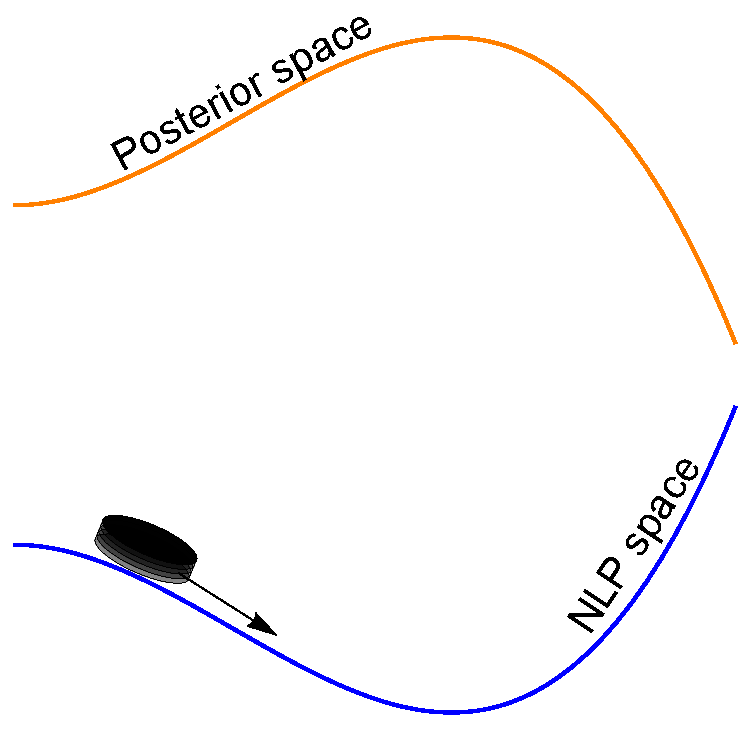
\includegraphics[width=0.3\textwidth]{./Figures/lec5_icePuck.pdf}}
	\end{figure}
	
	Hamilton in Monte Carlo.
	
	\begin{figure}[ht]
		\centerline{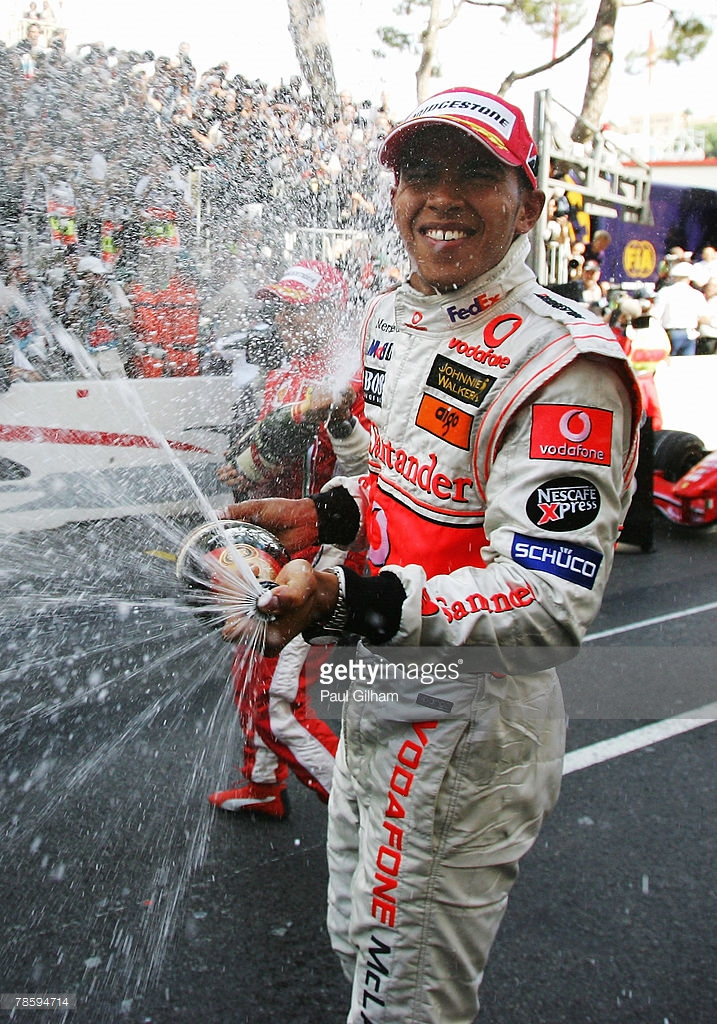
\includegraphics[width=0.3\textwidth]{./Figures/hamiltonMonteCarlo1.jpg}}
	\end{figure}
	
	
\end{frame}

\end{document}

